\documentclass[10pt,twocolumn]{article} 
\usepackage{simpleConference}
\usepackage{times}
\usepackage{graphicx}
\usepackage{amssymb}
\usepackage{url,hyperref}
\usepackage{tikz}

\begin{document}

\title{PhD Transfer Report}

\author{Conor Mc Keever \\
\today\\
conor.mckeever.16@ucl.ac.uk\\
}

\maketitle
\thispagestyle{empty}
\tableofcontents
\section{Introduction}
\subsection{quantum simulation}
In many fields of science strong correlations play an important role analyzing models of various phenomena. When classical numerical methods fail to be efficient tools for solving these problems, quantum simulators offer a promising alternative. The basic idea of a quantum simulator is to map a problem of interest to the Hamiltonian of a physical platform which hosts strongly correlated quantum states. The solution to the problem may then be deduced from observables of the simulator, for instance the solution could be mapped to the ground state of the simulator. In the medium term - five to ten years - the applications of quantum simulators are set to range from those aimed at solving the most difficult problems in condensed matter physics to nuclear physics, high energy physics and cosmology [12]. In the longer term (> 10 years), it is hoped that quantum simulators will support the design of novel complex materials and aid in simulation of quantum dynamics and chemical reactions in order to facilitate drug design [11].

With these applications in mind, one of the most active branches of quantum technologies has been the development of physical platforms suitable for quantum simulation. To date, such physical systems have included platforms from cold atoms [13] to photonic based systems [22] and they have seen success in the simulation of condensed matter phenomena including many body localization, topological quantum matter and out  of equilibrium dynamics. Moreover, state of the art quantum simulators habe recently been able to impose abelian and non-abelian gauge fields allowing for the study of toy models of quantum field theories which are may help solve important open problems in high energy physics. These are however a number of obstacles which many of these simulation platforms encounter, these include the difficulty of dissipating energy from the devices in order to reach low energy states, barriers to scalability, access to information and the presence of unwanted disorder. 

In this project we focus on photonic quantum simulators. These are physical platforms in which strong correlations are generated between photons generally via interaction with matter. In particular we are interested in polariton lattices and cavity QED systems. The central aim of the project is to develop classical numerical methods to simulate phenomena which may be simulable on these platforms and to guide experimental realization and verification of these devices.

Changsuk Noh 1,2 and Dimitris G. Angelakis 1,3

\subsection{polariton lattices}
Microcavity polaritons are light-matter quasiparticles with remarkable non-linear properties. With an effective mass on the order of 10 −5 m e , quantum effects in these quasiparticles can persist in these systems even up to room temperature [5]. Recently, a new candidate platform for quantum simulation has emerged. Polariton lattices are one- or two-dimensional arrays of semiconductor microcavities which host polaritons with properties which could overcome some of the barriers of conventional simulation platforms and make strides towards simulators which could operate on-chip and at relatively high temperatures.

Polariton lattices have already been realised experimentally using a number of methods. These include open cavities, micropillar arrays and surface acoustic waves (SAWs) [5]. The main advantages as compared to other platforms are that the observation of photoluminescence allows for easy access to information, while energy resolved detection allow access to ground state of the system as well as the whole excitation spectrum. Furthermore single lattice site resolution is possible with spatially resolved measurements allowing for the study of ordering phenomena. Conservative dynamics can be studied on timescales within the polariton lifetime while on longer timescales, the inherent driven-dissipative nature of polariton lattices make them an ideal simulator of correlated and topological states in the presence of dissipative and non-equilibrium conditions [1].

As it stands the main limitation of these devices is in the generation of strong correlations between polaritons however significant efforts are being made experimentally to overcome this, moreover disorder as a result of imperfections in fabrication can lead to some uncertainty in measurements...
 
\subsection{cavity QED}


\subsection{existing numerical methods}
There exist a number of methods to numerically solve strongly correlated quantum many-body systems. These include exact diagonalisation (ED), Quantum montecarlo methods (QMC) and [A few others] among others. Each of these methods have their respective advantages and disadvantages and a thorough numerical analysis of a model typically employs a number of cemplimentary methods. [write about the advantages and disadvantes of each]  



\subsection{proposed solutions}
Propose the solution of tensor network methods in and out of equilibrium. MPS, PEPS and iPEPS. State why this is a good choice to investigate phenomena we are interested in. Driven-dissipative phase transitions and topological states. 
\subsection{outline of report}
This can be done at the end. 

\section{Literature Review}
\subsection{standard introduction to tensor networks}
In tensor network methods, the wave function of a quantum many body state is paramaterised by a set of interconnected tensors. The central motivation is to use this parameterisation to restrict the states of the wave fucntion to a subspace of the full many-body Hilbert space and thereby circumvent the intractable task of representing it exactly. Remarkably, this subspace sometimes dubbed the \textit{physical corner of Hilbert space} - allows for the efficient representation of a large class of states of interest. For instance, it is known that ground states of 1D gapped Hamiltonians can be well approximated by matrix product states (MPS).  An intuitive understanding of this was put forward by Hastings. If the growth of entanglement entropy across a bipartition of a 1D state of a quantum system obeys an area law then that state can be well represented by an MPS.  Low entanglement states admit an efficint TN representation. 

The MPS is one example of a host of tensor network anzatze which have been developed over recent years. Others include the multiscale entanglement renormalization anzats (MERA) and projected entangled pair states (PEPS) among others. In this work we focus on the PEPS anzats which has been used to represent many-body wave functions in 2D geometries.  

\subsection{introduce PEPS, iPEPS and properties}

\begin{figure}
    \centering
    
\tikzset{every picture/.style={line width=0.75pt}} %set default line width to 0.75pt        

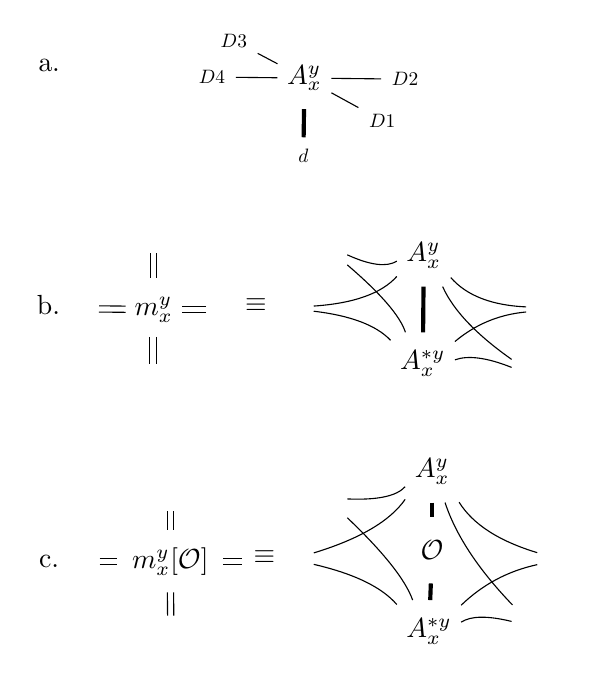
\begin{tikzpicture}[x=0.75pt,y=0.75pt,yscale=-1,xscale=1]
%uncomment if require: \path (0,539.6000003814697); %set diagram left start at 0, and has height of 539.6000003814697


% Text Node
\draw (152.03,65.47) node   {$A^{y}_{x}$};
% Text Node
\draw (189.5,86) node [scale=0.7]  {$D1$};
% Text Node
\draw (200.5,66) node [scale=0.7]  {$D2$};
% Text Node
\draw (118,47.5) node [scale=0.7]  {$D3$};
% Text Node
\draw (107.5,65) node [scale=0.7]  {$D4$};
% Text Node
\draw (151.5,103) node [scale=0.7]  {$d$};
% Text Node
\draw (209.53,150.97) node   {$A^{y}_{x}$};
% Text Node
\draw (260.83,207.83) node [scale=0.7]  {$$};
% Text Node
\draw (267.83,176.67) node [scale=0.7]  {$$};
% Text Node
\draw (163.67,147.33) node [scale=0.7]  {$$};
% Text Node
\draw (147.5,176.33) node [scale=0.7]  {$$};
% Text Node
\draw (209.03,202.97) node   {$A^{*y}_{x}$};
% Text Node
\draw (213.53,254.97) node   {$A^{y}_{x}$};
% Text Node
\draw (260.83,328.83) node [scale=0.7]  {$$};
% Text Node
\draw (273.17,297.33) node [scale=0.7]  {$$};
% Text Node
\draw (163.67,268.33) node [scale=0.7]  {$$};
% Text Node
\draw (147.5,297.33) node [scale=0.7]  {$$};
% Text Node
\draw (212.03,331.97) node   {$A^{*y}_{x}$};
% Text Node
\draw (213.53,292.97) node   {$\mathcal{O}$};
% Text Node
\draw (79.37,176.97) node   {$m^{y}_{x}$};
% Text Node
\draw (113.7,176.97) node   {$$};
% Text Node
\draw (44.03,176.63) node   {$$};
% Text Node
\draw (79.37,137.3) node   {$$};
% Text Node
\draw (79.03,173.63) node   {$$};
% Text Node
\draw (128.67,175) node   {$\equiv $};
% Text Node
\draw (87.37,298.3) node   {$m^{y}_{x}[\mathcal{O}]$};
% Text Node
\draw (130.7,298.3) node   {$$};
% Text Node
\draw (44.37,298.3) node   {$$};
% Text Node
\draw (87.37,261.63) node   {$$};
% Text Node
\draw (87.7,340.97) node   {$$};
% Text Node
\draw (132.67,296.33) node   {$\equiv $};
% Text Node
\draw (79.03,215.97) node   {$$};
% Text Node
\draw (29,59.67) node  [align=left] {a.};
% Text Node
\draw (28.67,174.67) node  [align=left] {b.};
% Text Node
\draw (29,298.33) node  [align=left] {c.};
% Connection
\draw    (129.5,53.57) -- (139.03,58.6) ;


% Connection
\draw    (189,65.87) -- (165.03,65.61) ;


% Connection
\draw    (119,65.12) -- (139.03,65.33) ;


% Connection
\draw    (165.03,72.59) -- (178,79.7) ;


% Connection
\draw [line width=1.5]    (151.63,94) -- (151.82,80.47) ;


% Connection
\draw    (172.67,150.65) .. controls (183.67,155.67) and (191.62,156.69) .. (196.53,153.7) ;


% Connection
\draw    (258.83,175.72) .. controls (242.2,174.99) and (230.1,170.29) .. (222.53,161.6) ;


% Connection
\draw    (156.5,175.33) .. controls (175.88,174.01) and (189.22,169.24) .. (196.53,161.03) ;


% Connection
\draw    (218.6,165.97) .. controls (223.69,177.32) and (234.76,189) .. (251.83,201.01) ;


% Connection
\draw    (172.67,155.49) .. controls (188.84,169.35) and (198.18,180.18) .. (200.67,187.97) ;


% Connection
\draw [line width=1.5]    (209.39,165.97) -- (209.18,187.97) ;


% Connection
\draw    (156.5,177.81) .. controls (174.37,179.93) and (186.72,184.61) .. (193.53,191.84) ;


% Connection
\draw    (258.83,178.18) .. controls (245.86,179.35) and (234.43,184.09) .. (224.53,192.41) ;


% Connection
\draw    (251.83,204.88) .. controls (239.96,200.15) and (230.86,198.94) .. (224.53,201.23) ;


% Connection
\draw    (172.67,268.25) .. controls (187.17,268.88) and (196.46,266.91) .. (200.53,262.35) ;


% Connection
\draw    (264.17,294.13) .. controls (245.7,288.56) and (233.16,280.46) .. (226.53,269.83) ;


% Connection
\draw    (156.5,294.26) .. controls (178.58,287.52) and (193.26,278.92) .. (200.53,268.47) ;


% Connection
\draw    (219.75,269.97) .. controls (224.92,285.7) and (235.75,302.15) .. (252.26,319.33) ;


% Connection
\draw    (172.67,277.31) .. controls (190.16,293.98) and (200.66,307.2) .. (204.15,316.97) ;


% Connection
\draw    (156.5,299.77) .. controls (175.91,304.26) and (189.25,310.71) .. (196.53,319.13) ;


% Connection
\draw    (264.17,299.91) .. controls (250.06,302.96) and (237.84,309.48) .. (227.53,319.45) ;


% Connection
\draw    (251.83,327.27) .. controls (240.24,324.44) and (232.14,324.55) .. (227.53,327.62) ;


% Connection
\draw [line width=1.5]    (213.53,269.97) -- (213.53,276.97) ;


% Connection
\draw [line width=1.5]    (212.92,308.97) -- (212.61,316.97) ;


% Connection
\draw    (104.7,178.47) -- (92.87,178.47)(104.7,175.47) -- (92.87,175.47) ;


% Connection
\draw    (53.05,175.22) -- (65.88,175.34)(53.02,178.22) -- (65.85,178.34) ;


% Connection
\draw    (80.87,149.8) -- (80.87,161.97)(77.87,149.8) -- (77.87,161.97) ;


% Connection
\draw    (121.7,299.8) -- (112.87,299.8)(121.7,296.8) -- (112.87,296.8) ;


% Connection
\draw    (53.37,296.8) -- (61.87,296.8)(53.37,299.8) -- (61.87,299.8) ;


% Connection
\draw    (88.87,274.13) -- (88.87,283.3)(85.87,274.13) -- (85.87,283.3) ;


% Connection
\draw    (88.98,313.29) -- (89.07,324.45)(85.98,313.31) -- (86.07,324.48) ;


% Connection
\draw    (80.53,190.13) -- (80.53,203.47)(77.53,190.13) -- (77.53,203.47) ;



\end{tikzpicture}

    \caption{a. iPEPS tensor labelled with the set of bond dimesions $\{D1,D2,D3,D4\}$ and the physical dimension $d$. b. Tensor ntwork diagram of the contraction used to find the transfer tensor $m_x^y$ from the iPEPS $A^y_x$. c. Calculation of an observable using its matrix representation $\mathcal{O}$, the physical indices $d$ are contracted over. }
    \label{fig:my_label}
\end{figure}
\begin{figure}
    \centering
    \vspace{1cm}

\tikzset{every picture/.style={line width=0.75pt}} %set default line width to 0.75pt        

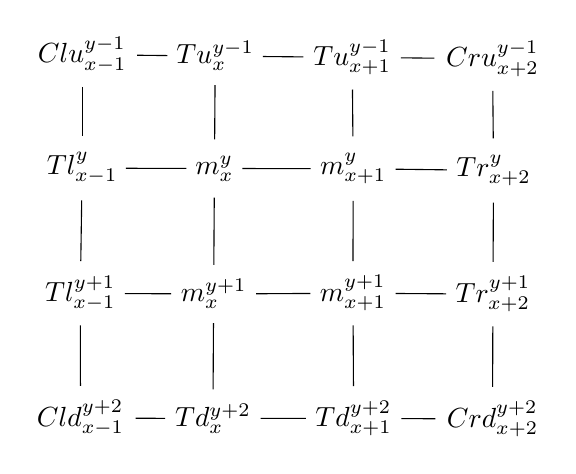
\begin{tikzpicture}[x=0.75pt,y=0.75pt,yscale=-1,xscale=1]
%uncomment if require: \path (0,503); %set diagram left start at 0, and has height of 503

% Text Node
\draw (187.37,86.03) node   {$m^{y}_{x+1}$};
% Text Node
\draw (120.53,85.97) node   {$m^{y}_{x}$};
% Text Node
\draw (120.13,146.43) node   {$m^{y+1}_{x}$};
% Text Node
\draw (187.27,146.03) node   {$m^{y+1}_{x+1}$};
% Text Node
\draw (120.9,31.8) node   {$Tu^{y-1}_{x}$};
% Text Node
\draw (186.9,32.4) node   {$Tu^{y-1}_{x+1}$};
% Text Node
\draw (187.6,206.3) node   {$Td^{y+2}_{x+1}$};
% Text Node
\draw (119.8,206.4) node   {$Td^{y+2}_{x}$};
% Text Node
\draw (255,86.9) node   {$Tr^{y}_{x+2}$};
% Text Node
\draw (254.7,146.5) node   {$Tr^{y+1}_{x+2}$};
% Text Node
\draw (56.8,85.8) node   {$Tl^{y}_{x-1}$};
% Text Node
\draw (55.9,146.1) node   {$Tl^{y+1}_{x-1}$};
% Text Node
\draw (56.8,31.1) node   {$Clu^{y-1}_{x-1}$};
% Text Node
\draw (254.5,33.1) node   {$Cru^{y-1}_{x+2}$};
% Text Node
\draw (254.5,206.7) node   {$Crd^{y+2}_{x+2}$};
% Text Node
\draw (56,206.2) node   {$Cld^{y+2}_{x-1}$};
% Connection
\draw    (134.03,85.98) -- (166.87,86.01) ;


% Connection
\draw    (120.44,99.97) -- (120.23,132.43) ;


% Connection
\draw    (140.63,146.31) -- (166.77,146.16) ;


% Connection
\draw    (187.34,101.53) -- (187.29,130.53) ;


% Connection
\draw    (83.3,31.39) -- (97.9,31.55) ;


% Connection
\draw    (143.9,32.01) -- (163.4,32.19) ;


% Connection
\draw    (210.4,32.64) -- (226.5,32.81) ;


% Connection
\draw    (77.8,85.85) -- (107.03,85.93) ;


% Connection
\draw    (77.4,146.21) -- (99.63,146.33) ;


% Connection
\draw    (207.87,86.3) -- (232.5,86.61) ;


% Connection
\draw    (207.77,146.18) -- (232.2,146.34) ;


% Connection
\draw    (82.5,206.28) -- (96.8,206.33) ;


% Connection
\draw    (142.8,206.37) -- (164.6,206.33) ;


% Connection
\draw    (210.6,206.44) -- (227,206.54) ;


% Connection
\draw    (56.8,46.6) -- (56.8,70.3) ;


% Connection
\draw    (56.57,101.3) -- (56.13,130.6) ;


% Connection
\draw    (55.93,161.6) -- (55.97,190.7) ;


% Connection
\draw    (120.81,45.8) -- (120.63,71.97) ;


% Connection
\draw    (120.06,160.43) -- (119.88,192.4) ;


% Connection
\draw    (187.35,161.53) -- (187.51,190.8) ;


% Connection
\draw    (187.03,47.9) -- (187.23,70.53) ;


% Connection
\draw    (254.64,48.6) -- (254.86,71.4) ;


% Connection
\draw    (254.92,102.4) -- (254.78,131) ;


% Connection
\draw    (254.65,162) -- (254.55,191.2) ;



\end{tikzpicture}
    \caption{A $2 \times 2$  cell of transfer tensors $\{m^y_x\}$ surrounded by its environment. } 
    \label{fig:my_label}
\end{figure}
\subsection{important relevant work related to equilibrium PEPS}
\subsection{important relevant work related to out of equilibrium PEPS}



\section{Work Completed}
\subsection{iPEPS Algoritm}


\subsection{iPEPO Algorithm}

\section{Initial Results and Benchmarks}

\subsection{Ground State of Transverse Quantum Ising Model}
The transverse Ising Model is commonly used to benchmark numerical methods of this type. Here we benchmark our algorithm against that in the literature by finding the ground state of the transvere Ising model Hamiltonian for a range of parameters which exhibit a phase transition. The benefit of benchmarking by plotting a phase diagram is that the critical value of the particular order parameter in question can be compared easily with values from the literature. Here we find the ground state of the 2D ising model on a square lattice which is described by the hamiltonian:
 \begin{equation}
 H = J_z \sum_{\langle i,j \rangle} \sigma_i^z \sigma_j^z + h_x \sum_{i} \sigma_i^x
 \end{equation}
 The algorithm proceeds as follows 
 
\begin{enumerate}
\item A value for the iPEPS bind dimension $D$ is chosen and a set of four random initial iPEPS tensors $\{a,b,c,d\}$ are created which define a 2$\times$2 unit cell.
\item A value for the imaginary time-step $\delta t$ is chosen and the two-body Hamiltonian gates $H_{\langle i,j \rangle}$ are constructed.  
\item The simple update procedure is applied to each bond of the unit cell as desciribed in section [SECTION]. 
\item Step 3. is apllied iteratively for some chosen value $N \sim 1000$
\item A new, smaller value of $\delta t$ is chosen and steps 2 to 4 are repeated.  
\item Step 5 is repeated until a minimum chosen $\delta t \sim 10^{-5}$ is reached. 
\item An appropriate value of $\chi$ is chosen and the set of transfer matrices $\{ma, mb, mc,md\}$ and environment tensors $\{Clu,Cru,Cld,Crd, Tu,Tr,Tl,Td\}$  are constructed according to the procedure in section [SECTION]
\item The environemnt tensors are renormalised iteratively according the procedure described in section [SECTION] until convergence is reached. 
\item The value of local observables are then caluclated and saved.
\end{enumerate}

 \begin{figure}[h]
    \centering
    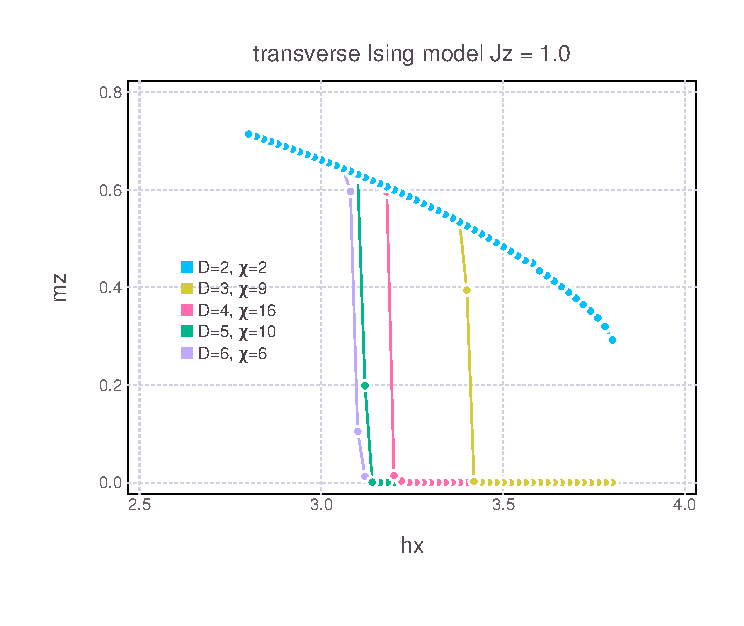
\includegraphics[width= \linewidth]{IsingBenchmarkingSmall.pdf}
    \caption{The magnetization $m_z= \lvert \sigma _z \rvert$ as a function of the transverse field $h_x$ for the ground state of the transverse Ising model with $J_z = 1.0$. A range of values of the iPEPS bond dimension $D$ and environment bond dimension $\chi$ reveal better approximations of the critical field $h_x^c$ with increasing $D$. }
    \label{fig:my_label}
\end{figure}

To evidence the phase transition we calculate the value of $m_z = \lvert \langle \sigma_z \rangle \rvert$ for a range of values of the transvere field $h_x$. The current best estimate for the critical value of the transverse field $h_x^c$ is $h_x^c = [FIND]$ [reference ]. Figure [FIGURE] shows the results of our benchmarking for a range of choices of the iPEPS bond dimension $D$ and the environment bond dimension $\chi$. As the value of $D$ is increased, $h_x^c$ is found to converge to a better and better approximation of the literature value. The chosen value of $\chi$ in each case has little impact on $h_x^c$ (see Figure [FIGURE ] in SUPINFO), hovever its impact is more readily aboserved in the calculation of other observables such as correlations [CHECK IF THIS IS CORRECT]. In practice, larger values of $\chi$ should be chosen to ensure the environment tensors provide an accurate approximation of the actual environment. In this respect, an appropriate method of diciding upon convergence of the environment tensors is currently being worked and could for instance be based on the convergence of nearst neighbour correlations. 

\subsection{Steady State of Dissipative Transverse Quantum Ising Model}


\section{Plan for Future Work}


This material is important -- part of the value of a paper is showing how the work sets new research directions. I like bullet lists here. A couple of things to keep in mind:
\begin{description}
  \item[$\bullet$]  If you're actively engaged in follow-up work, say so. E.g.: ``We are currently extending the algorithm to... blah blah, and preliminary results are encouraging." This statement serves to mark your territory.
\item[$\bullet$]  Conversely, be aware that some researchers look to Future Work sections for research topics. My opinion is that there's nothing wrong with that -- consider it a compliment.
\end{description}


\section{Appendix A}
This is a simple sample of a document created using \LaTeX
   (specifically pdflatex) that includes a figure from the Vergil visual editor for Ptolemy II
   that was created by printing to the Acrobat Distiller to get a PDF file.
   It also illustrates a simple two-column conference paper style,
   and use of bibtex to handle bibligraphies.

This is a sample document for use with pdflatex, which is
a program that is included with the Miktex distribution
that directly produces PDF files from \LaTeX sources.
To run \LaTeX on this file, you need the following files:
\begin{enumerate}
\item templatePDF.tex (this file)
\item figure.pdf (the figure file)
\item simpleConference.sty (style file)
\item refs.bib (bibiliography file)
\end{enumerate}
\noindent
To create a PDF file, execute the following commands:
\begin{enumerate}
\item pdflatex mainTemplatePDF
\item bibtex mainTemplatePDF
\item pdflatex mainTemplatePDF
\item pdflatex mainTemplatePDF
\end{enumerate}
\noindent
Yes (strangely) it is necessary to run pdflatex three times.
The result will be a PDF file (plus several other files that \LaTeX
produces).  You will need a mechanism, of course, for executing
commands on the command line. If you are using Windows, I recommend
installing Cygwin and using its bash shell.








\section{Appendix B: How to Include Vergil Diagrams as Figures}

\cite{PtolemyVol1:04}


\bibliographystyle{abbrv}
\bibliography{refs}
\end{document}
